\chapter{The cross-platform compendium creation methodology and COMMAND 
system}\label{ch:command}
\chaptermark{Command}

\ldots

\instructionsintroduction

\section{Introduction}

Microarrays are one of the main technologies for large-scale transcriptional 
gene expression profiling. 
To promot data sharing, scientific journals generally require the 
deposit of these high-throughput experiments in public databases, such as Gene 
Expression Omnibus (GEO) \cite{Barrett2011} or ArrayExpress 
\cite{Parkinson2009}, upon publication. 
These databases are an extremely rich source of information, containing freely 
accessible data for thousands of experiments and a multitude of different 
organisms, and in theory provide an opportunity to analyse gene expression of a 
particular species at a global level. 
They hold the potential to expand the scope of any smaller scale study: 
mining the information contained in such databases offers molecular biologists 
the possibility to view their own dedicated experiments and analysis in light 
of what is already available. 
So far however, this wealth of public information remains largely untapped 
because these databases do not allow for a direct and integrated exploration of 
their data. 
The opportunity of combining all public experiments for a single organism has 
not been explored due to practical issues that can ultimately be attributed to 
the large heterogeneity inherent to microarray data. 
Data sets originate from different experimenters or labs and microarrays do not 
constitute a uniform technology. 
Multiple microarray platforms exist and are manufactured in different ways. 
Even for similar platforms, protocols for sample preparation, labelling, 
hybridization and scanning can vary greatly. 
Although community standards specifying the mandatory minimal experimental 
information accompanying each dataset (e.g., MIAME \cite{Brazma2001}) have been 
long established, the lack of the requirements \cite{Brazma2009} imposed 
regarding the format of the platform descriptions and the expression 
measurements, as well as the degree of preprocessing done on these values 
further complicates the matter of experiment integration from a practical point 
of view. 


Despite such difficulties, several initiatives exist to actively build 
expression compendia from public resources. 
Most existing compendia can roughly be divided in two groups \cite{Fierro2008}: 
those that directly integrate single-platform experiments, and those that 
indirectly integrate cross-platform experiments. 
Combining data from a single platform makes the in-between experiment 
normalization and probe mapping relatively straightforward, so that 
the quantitative measures of gene expression can be analysed directly across 
experiments. 
Most single-platform compendia databases, such as for instance 
M$^{\textrm{3D}}$ \cite{Faith2008}, or the commercial Genevestigator 
\cite{Hruz2008}, focus on Affymetrix, one of the more robust and reproducible 
platforms \cite{Bammler2005, Irizarry2005}. 
Combining data from different platforms, even to the extent of combining data 
from single- and dual-channel microarrays, is generally done by indirect 
meta-analysis as opposed to directly integrating the actual expression values: 
one first applies the desired analysis procedure (e.g., identifying 
differentially expressed genes, clustering gene expression profiles, etc.) on 
each single data set within the compendium separately, and subsequently 
combines the derived results. 
These compendia are often topic-specific, collecting all publicly available 
experimental information related to a subject matter of interest. 
ITTACA \cite{Elfilali2006} and ONCOMINE \cite{Rhodes2007}, for instance, focus 
on cancer in human; Gene Aging Nexus \cite{Pan2007} on aging in several 
species. 
There are exceptions though, such as the large ATLAS \cite{Kapushesky2010} 
initiative from ArrayExpress.


The compendia created by directly integrating data across experiments have the 
advantage of retaining actual expression values, which broadens the scope of 
potential analysis procedures compared to indirect meta-analysis.
Most of such compendia center on eukaryotic organisms, for which considerable 
amounts of data are available. 
Relying on only one platform can still lead to sizeable compendia with a broad 
scope in condition content, such as the human compendium constructed based on 
the Affymetrix U133A platform with over 5000 samples \cite{Lukk2010}. 
However, for most species (e.g., \textit{Zea mays}), no single platform has 
such a dominant role. 
%
The worst is prokaryotes. 
Even for model organisms such as {\it E. coli}, much less data is available on 
individual platform and a significant portion of the data is missed out when 
considering only one platform. 

To have the advantage of the direct integration, while not being limited to a 
single platform, we have devised methodology that directly combines 
expression data across platforms and experiments. 
The methodology has enabled us to create comprehensive compendia incorporating 
most high quality public data covering a broad range of experimental 
conditions as well as extensive types of biological samples. 
To facilitate the creation of new compendium and the curation of the existing 
ones, a software system COMMAND (Cross-platform cOMpendium MANagement Desktop) 
is also developed, utilizing web browser as the front-end and our methodology 
at the back-end. 







\section{Methods}

\textbf{Hurdles to create cross-platform exp compendium}

There are \textbf{three main hurdles} preventing direct data integration across 
platforms and experiments.

\begin{itemize}

\item[exp-data]
The lack of a consistent format to report expression data prevents an automatic 
and computerized data retrieve.
%
The heterogeneity of microarray platforms hampers direct integration 
in two aspect.
The possible probe sequence differences of a gene across different platforms 
questions the compatibilities of the obtained measurements.

\item[metadata]
The metadata describing biological sample and experimental 
conditions is provided as free text which is often incomplete and lack of 
consistency. 
Standards like MIAMI \cite{Brazma2001, Brazma2009}, although promote human 
interpretation of experimental conditions, do not facilitate computational 
analysis.

\item[normalization] 
The different preprocessing algorithms employed by different experiments 
further complicates the data compatibility.
%
The log ratio calculation, capable of removing certain technical variations 
from the normalized data, inherently improves the data consistency across 
platforms and experiments \cite{Shi2006, Shi2008}

\end{itemize}



\subsection{Cross-platform expression compendion}

Our expression compendium is essentially an organism-specific matrix of 
expression values derived from publicly available microarray experiments which 
are homogenized to make them comparable. 
The rows of a compendium correspond to the known genes of the organism 
in question. 
Uniquely, each column of it is a `\textit{condition contrast}', which 
does not represent single biological sample, but in fact always represent the 
difference between a pair of samples, one as test and the other reference. 
Consequently, the expression values themselves are calculated as expression 
log-ratios. 
Converting absolute measurements of expression into expression changes is the 
principal means for rendering expression values comparable across platforms and 
experiments. 
Relative expression calculated intra-experiment/platform (i.e. between two 
conditions measured in the same microarray experiment using one platform) 
negates much of the platform and experiment specific variations that makes it 
impossible to reliably compare the absolute quantities reported in different 
experiments \cite{Shi2006}.



\subsection{Cross-platform expression compendion creation methodology}
\label{sec:colombos-comp-method}

\begin{figure}
	\centering
  	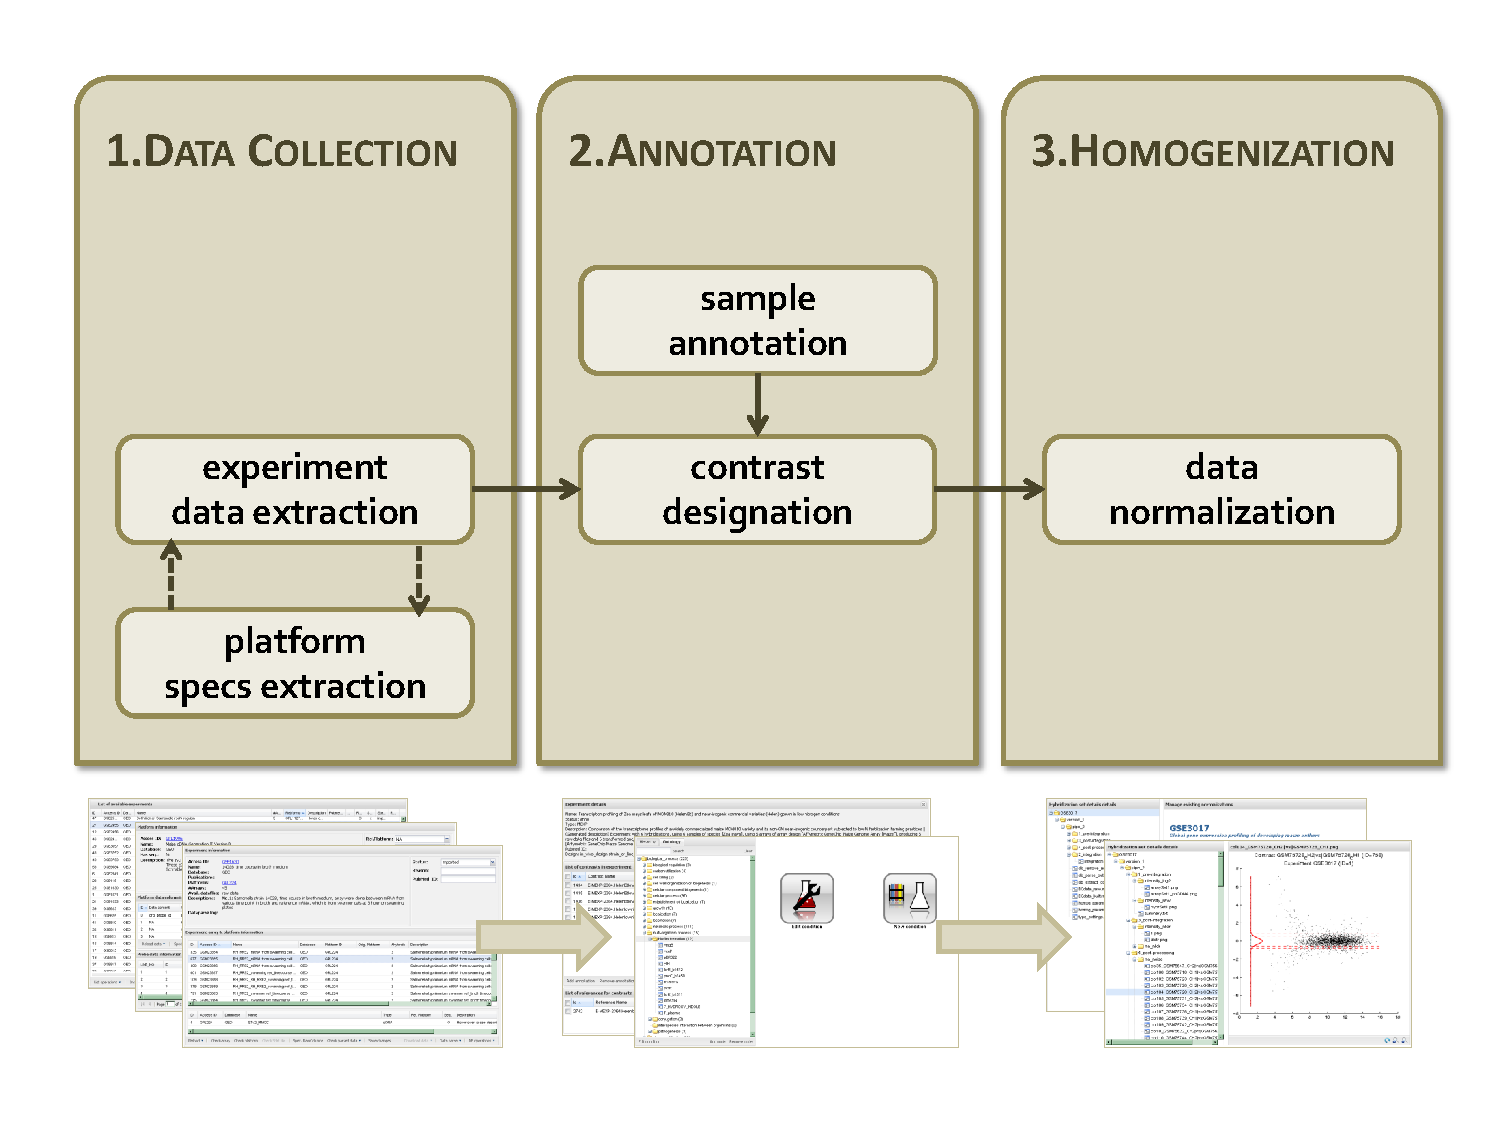
\includegraphics[width=1\textwidth]{COMMAND_Workflow.pdf}
  	\caption[Cross-platform expression compendium creation methodology]{
  	\textbf{Cross-platform expression compendium creation methodology}.
  	 From left to right, three box represent three main steps of the 
  	 cross-platform expression compendium creation methodology. The 
  	 corresponding functionalities are specified in the rectangles inside of 
  	 each box. Below the box shown the snapshots of the corresponding COMMAND 
  	 interfaces.}
  	\label{fig:command-workflow}
\end{figure}


The cross-platform compendium creation methodology is composed of three major 
steps (Figure \ref{fig:command-workflow}), namely, data collection, experiment 
annotation, and data homogenization. 
%
First, in data collection step, the expression data and the accompany 
(experiment and platform) information are retrieved from the online 
repositories, overcoming the issue of the prevalent data representation 
discrepancies. 
%
Next in annotation step, the contrasts are constructed by assigning a pair of 
samples, one as reference and the other as test. And the experimental 
condition differences between the corresponding samples are 
curated manually and specified for each contrast using a set of in-house 
controlled vocabularies.
%
At last, the raw expression data are normalized and converted into log 
ratios based on the sample contrast association in data homogenization step, 
creating a cross-platform expression compendium.
% 
% 
In the following sections, we will explain the individual step in detail.



\subsection{Data collection}


\begin{itemize}
\item handle various expression data reporting format
\item handle various platforms, probe annotation
\end{itemize}

Huge amount of gene expression experiment data are publicly available 
at online repositories such as GEO and ArrayExpress. 
 
holds hundreds even 
thousands 
of experiments for each species, 

To create a compendium, the data need to be collected 



The first step is the retrieval of microarray experiments and associated 
platforms from Gene Expression Omnibus (GEO) and ArrayExpress. 
Representation discrepancies prevalent in experimental data directly obtained 
from online databases are systematically removed and the resulting data are 
then stored as available in a uniform format. 
`As available' does not necessarily equate to raw scanner output, since there 
are no MIAME reporting standards regarding the measurement units of expression 
\cite{Brazma2001, Brazma2009}. 
Often raw intensities are not provided in the public databases (especially for 
older experiments), and only already processed data are reported. 

At this stage probes are also mapped in a platform-specific manner to a unique 
list of genes which is constructed based on the organism's RefSeq file at NCBI 
\cite{Pruitt2007} and which corresponds to the rows of the final compendium. 
If probe sequences are available or can be obtained from the platform 
description, the mapping is driven by sequence homology searches using 
BLAST \cite{Altschul1997}. 
If not, a probe's target gene is identified by other probe info, namely -and in 
order of preference: locus tags, alternative gene tags, or common gene names.


\textbf{General workflow}

Figure


\subsection{Annotation}


\begin{itemize}
\item manual curation
\item controlled vocabulary
\item hierarchy (classification)
\item ontology (functional connection)
\end{itemize}



In a next phase, the condition contrasts that will be represented in the 
compendium are defined and annotated. Based on their biological role in an 
experimental survey, hybridizations are labelled `reference' or `test' on a per 
experiment-and-platform combination basis and matched to produce a set of 
condition contrasts. For a single channel experiment, one or more 
hybridizations are chosen as references for the remaining tests. For dual 
channel experiments, usually one of every two array
hybridizations serves as a reference to the other, as this inherently counters 
much probe spot associated variation in the measurements. There are exceptions 
however, such as when one of the hybridizations on an array does not constitute 
an identifiable and unique biological condition for which the transcriptome was 
assessed (e.g. a sample of genomic DNA or a pool of different samples that 
cannot be considered as biological replicates). These hybridizations are 
discarded and the experiment is further treated as if it was a single channel 
experiment. In this way we ensure that every contrast has a biologically 
interpretable meaning: its associated log-ratios measure changes in expression 
in response to quantifiable stimuli that are altered from reference to test. 
Using a set of formal hierarchically structured condition properties 
(representing for instance mutations, compounds in the growth medium, 
treatments, and general growth conditions), we can then specify the annotation 
of each condition contrast rigidly as a vector representing the differences for 
these property values between the test and reference condition. This 
representation enables a mathematical comparison and automatic organization of 
contrasts based on the conditions that are surveyed, but it is a labor 
intensive manual curation process where information often needs to be retrieved 
from original publications, supplementary data and occasionally directly from 
the authors. The condition properties themselves are further structured in a 
condition ontology tree. This ontology employs the same classes as the Gene 
Ontology biological process subtree terms \cite{Gene2010} and maps the 
condition properties used to annotate the condition contrasts to one or more 
biological processes or functionalities they most likely affect.


\textbf{From Oncomine3 paper \cite{Rhodes2007}} p2 
//
Because micro-
array data are only as valuable as the sample information
accompanying them, our data collection team places special
emphasis on sample facts curation and standardization. In
many cases, this permits us to test hypotheses not explored
in original analyses and publications
When
possible, sample facts are translated to standard terms used
by the NCI Thesaurus [10], allowing us to provide definitions
for clinical terms.


\subsection{Data homogenization}

\begin{itemize}
\item consistent per experiment normalization across
\item log ratio calculation
\end{itemize}



The final part in the creation of a compendium is the homogenization of the 
expression data: several preprocessing procedures are conducted to render 
expression levels comparable between different experiments and platforms. 
Crucial steps in this preprocessing are array-specific and depend on both the 
technological platform that was used to perform the experiment, as well as on 
the reported units of expression and the type of normalizations that might have 
already been done. In general we adhere to the following principles: 1) 
whenever possible, raw intensities are preferred as data source over normalized 
data provided by the public repository, 2) no local background or mismatch 
probe correction procedures are performed to avoid an increase in intensity 
error variance for lower, less reliable intensity levels 
\cite{Ritchie2007,Engelen2006,Li2001}, 3) non-linear normalization techniques 
are performed to account for global inter-hybridization differences (e.g. loess 
fit to remove dye-related discrepancies on dual channel arrays \cite{Yang2002}, 
quantile normalization for high-density oligonucleotide experiments 
\cite{Bolstad2003}) and 4) log-ratios are created for single-channel data 
according to the condition contrast definitions and combined with the dual 
channel measurements.


\subsubsection{Experiment design}

Thesis Zhao Hui Section 2.2.2.1

\subsubsection{Quality Assessment}

Thesis Zhao Hui Section 2.2.2.2




\section{COMMAND, web based system for expression compendium creation}





\section{Results and Discussion}

\textbf{Discussion: }

\textbf{Check Introduction - Log-ratios and condition contrasts by 
\textit{kristof}}

log-ratio, contrast specification, condition hierarchy and ontology


\textbf{Result: }

Table of raw data collection

Table of data annotation





%%%%%%%%%%%%%%%%%%%%%%%%%%%%%%%%%%%%%%%%%%%%%%%%%%
% Keep the following \cleardoublepage at the end of this file, 
% otherwise \includeonly includes empty pages.
\cleardoublepage


% vim: tw=70 nocindent expandtab foldmethod=marker foldmarker={{{}{,}{}}}
